
%Getting on the Right Track: A project for optimised route allocation systems.
\documentclass[11pt]{article}
\usepackage[margin=1in]{geometry}

%This is for Visual Studio Code compiler only.
\usepackage{hyperref}
\hypersetup{
    pdftitle={Optimised Route Allocation System},
    pdfauthor={Rafael Kozal},
    pdfcreator={LaTeX},
    pdfproducer={LaTeX Engine} % Or omit to let the engine populate it automatically
}

% Core packages
\usepackage{amsmath,amssymb}
\usepackage{tikz-cd}
\usepackage{multicol}
\usepackage{booktabs}% For professional table lines (\toprule, \midrule, \bottomrule)
\usepackage{array}
\newcolumntype{L}[1]{>{\raggedright\arraybackslash}p{#1}}
\usepackage[backend=biber,style=authoryear]{biblatex}
\addbibresource{references.bib}
\usepackage[inline]{enumitem} % for inline lists and customisation of enumeration
\usepackage[title]{appendix} % so the title of appendix is appendix and not A
\usepackage{pdflscape}   % rotates a single page to landscape
\usepackage{longtable}   % lets a table span multiple pages
\usepackage{listings} %allows u to use code
\usepackage{verbatim}
\usepackage{xcolor} % colour different text (for code)
\usepackage[scaled=0.95]{inconsolata} % clean, modern monospace font
\usepackage{siunitx} %SI units 
\usepackage{realboxes} % for inline code grey boxes

\definecolor{codegray}{named}{lightgray} %for inline code grey
\newcommand{\code}[1]{\Colorbox{lightgray!30}{\texttt{#1}}} %if u do \code it will run


% VS Code-inspired code colouring and formatting
\definecolor{vscodebackground}{HTML}{1E1E1E}
\definecolor{vscodeforeground}{HTML}{D4D4D4}
\definecolor{vscodekeyword}{HTML}{C586C0}
\definecolor{vscodefunction}{HTML}{DCDCAA}
\definecolor{vscodevariable}{HTML}{9CDCFE}
\definecolor{vscodestring}{HTML}{CE9178}
\definecolor{vscodecomment}{HTML}{6A9955}
\definecolor{vscodeoperator}{HTML}{D19A66}
\definecolor{vscodelinenumber}{HTML}{858585}

\lstdefinestyle{vscode}{
    language=Python,
    backgroundcolor=\color{vscodebackground},
    basicstyle=\ttfamily\footnotesize\color{vscodeforeground},
    keywordstyle=\bfseries\color{vscodekeyword},
    stringstyle=\color{vscodestring},
    commentstyle=\color{vscodecomment},
    emph={RegisterTransitCallback,AddDimension,GetDimensionOrDie,enumerate,NodeToIndex,CumulVar,SetRange},
    emphstyle=\color{vscodefunction},
    emph=[2]{time_callback_index,routing,time_callback,time_dimension,location_idx,time_window,data,index,manager},
    emphstyle=[2]\color{vscodevariable},
    literate=
        {=}{{{\color{vscodeoperator}=}}}1
        {+}{{{\color{vscodeoperator}+}}}1,
    numbers=left,
    numberstyle=\tiny\color{vscodelinenumber},
    stepnumber=1,
    numbersep=10pt,
    frame=single,
    rulecolor=\color{black},
    framerule=0.9pt,
    framesep=7pt,
    xleftmargin=1.5em,
    framexleftmargin=1.2em,
    xrightmargin=0.5em,
    breaklines=true,
    breakatwhitespace=false,
    showstringspaces=false,
    columns=fullflexible,
    keepspaces=true,
    tabsize=4,
    captionpos=b
}


\usepackage{graphicx} %for images
\usepackage{float} % floating images
\usepackage{subcaption} %capions for two images
\captionsetup[subfigure]{labelformat=parens,subrefformat=parens}


% Paragraphs
\setlength{\parindent}{0pt}
\setlength{\parskip}{1\baselineskip}

\title{Optimised Route Allocation System\\\large Computer Science GCE A Level Non-Examined Assessment}
\author{Candidate Name: Rafael Kozal\\Centre Number: \rule{4cm}{0.4pt}\\Candidate Number: \rule{4cm}{0.4pt}}
\date{\today}

\begin{document}
\maketitle

\begin{center}
\textbf{Project Summary}
\end{center}

This project will design, develop, and evaluate an optimised route allocation system for an organisation such as a supermarket, courier business, or local delivery company. The system will help allocate deliveries to multiple drivers while attempting to minimise total travel distance, reduce inefficient routing, and respect real-world constraints such as vehicle capacity, route length, customer delivery time windows with respect to tolls.

The underlying optimisation problem is the Capacitated Vehicle Routing Problem with Time Windows, abbreviated CVRPTW. In this well-known computer science problem, a fleet of vehicles must visit a set of customer locations. Each vehicle has limited capacity, and each customer may only be served within a specified time period. Although finding a perfectly optimal solution can be computationally expensive for larger inputs, the project will aim to produce high-quality routes using algorithms and heuristics that are practical for a real delivery environment.

\newpage
\tableofcontents
\newpage    

\section{Introduction}

Many supermarkets and delivery-based companies must organise large numbers of daily deliveries. Each order has a destination, a demand value (such as weight or number of items), and often a delivery window. At the same time, each delivery vehicle has a maximum carrying capacity and each driver may only be able to travel for a limited distance or duration. If routes are planned manually, the process can be slow, inconsistent, and inefficient as such routes may lead to unnecessary fuel costs, late deliveries, underused vehicles, and increased pressure on staff (which may result in accidents).

The aim of this project is to create an optimised route allocation system that supports a delivery manager in assigning deliveries to drivers. The system will take a set of delivery requests and vehicle details as input, then generate routes that attempt to satisfy all constraints while keeping the overall route cost as low as possible. Route cost may include total distance, number of vehicles used, estimated travel time, or a combination of these factors. The final system should present the generated routes clearly so that a user can understand which deliveries have been allocated to each driver and in what order they should be completed.

This project is suitable for a Computer Science GCE A Level Non-Examined Assessment because it involves several important computational concepts. These include graph representation, data modelling, algorithm design, optimisation, validation, testing, and evaluation. Locations can be represented as nodes in a graph, while travel distances or times can be represented as weighted edges. The system can then apply a route construction method, such as a nearest-neighbour or savings-based heuristic, followed by improvement techniques to reduce inefficient journeys. Constraint checking will also be required to ensure that no route exceeds vehicle capacity, route length, or delivery time window limits.

The intended user is a delivery coordinator working for a supermarket or company that manages multiple delivery drivers. The user needs a system that is faster and more reliable than planning routes manually. The system should allow the user to enter, load, or edit delivery and vehicle data, generate optimised route allocations, and view the results in a clear format. If a delivery cannot be allocated because of the given constraints, the system should identify this clearly rather than producing an invalid route.

The project will focus on producing a functional and testable prototype rather than a commercial-scale logistics platform. The prototype will use a realistic sample dataset containing customer locations, demands, vehicle capacities, time windows, and route limits. The success of the project will be judged by whether the system can create valid routes, reduce total travel time compared with a simple baseline approach, and provide understandable outputs for the user.

\subsection{Problem Statement}

A delivery company needs to assign a set of deliveries to a limited number of vehicles. Each delivery has a location, demand, and delivery time window. Each vehicle has a maximum capacity and may have a maximum route length. The system must decide which deliveries should be assigned to each vehicle and the order in which they should be visited, while aiming to minimise route cost and avoid breaking any constraints.

\subsection{Project Aim}

The aim of this project is to develop an optimised route allocation system that can generate efficient and valid delivery routes for multiple drivers while respecting vehicle capacity, delivery time windows, and maximum route length constraints.

\subsection{Initial Objectives}
\label{Specification} % label for the spec of the project
\begin{itemize}
    \item Analyse the needs of a supermarket or delivery company that manages multiple vehicles and customer deliveries.
    \item Model the delivery network using suitable data structures, including customer nodes, vehicle records, demands, time windows, and distance or travel-time values.
    \item Design and implement an algorithm that constructs valid vehicle routes while checking capacity, time window, and route length constraints.
    \item Improve the generated routes using an optimisation technique or heuristic so that the system performs better than a basic baseline method.
    \item Provide a clear user interface or output format showing each driver's assigned route, delivery order, total load, and route distance or duration.
    \item Test the system using normal, boundary, and erroneous data to confirm that constraints are handled correctly.
    \item Evaluate the final system against the project aim, user requirements, and measurable performance criteria.
\end{itemize}

\newpage
\section{Analysis}

\subsection{Background}
\label{sec:background}
Over the past few decades, the world has bared witness to a surge in globalisation, which has given society a greater access to products from around the world, faster communication, new opportunities, and more convenient ways of living. With just a few clicks, we can now order almost anything and have it delivered to our doorstep. Specifically, Dubai and the wider UAE have seen an exponential growth in deliveries of parcels including food, groceries and e-commerce. Platforms such as Talabat, Noon, Careem, Deliveroo and newer entrants (Keeta) have driven an expansion of last-mile logistics, with estimates stating tens of thousands of workers are working in the sector nationwide, and around 80,000+ working across logistics and delivery ecosystem as a whole. This growth can be accredited towards the high smartphone penentration, on-demand consumer expectation and the post-pandemic normalisation of online ordering.\cite{taxfreesalariesDelivery}

Despite this demand, delivery drivers occupy the lower end of the UAE wage distribution. Aggregated salary data places typical delivery driver earnings in the range of about AED 2,500-4,500 per month, with many roles clustering around AED 3,000-3,500. In practice, riders often work 10-12 hour shifts, six days a week, to achieve these figures, either on fixed salaries with performance bonuses or on a commission-only model where they are paid per completed order. Commission rates reported in the UAE commonly fall between roughly AED 7.5 and AED 10 per trip, aligning with riders' own accounts of “7-9 dirhams an order,” and requiring roughly 15-20 deliveries per day merely to break even after covering fuel, food, accommodation, and visa or agency fees.\cite{indeed_delivery_driver_dubai}

This creates a downstream risk which creates systemic penalties and saftey vulnerabilities. There is a transfer of financial and operational risk onto the driver, as compensation is preformance-oriented or proportional to order volume, time becomes a rider's currency. Any unexcpected delays (whether from traffic congestion, resturant preperation latency or gated community security checks) directly decrease their hourly wage and risk a defecit by pushing them below a financial break-even threshold needed to cover operational costs - fuel, bike leases and living costs. This economic strucutre creates a high pressure environment and feedback loop that directly incentives high risk behaviours on the road. \cite{roadsafetyuae_gig_pay_2024}

\begin{enumerate}
  \item Algorithmic pressure and customer ratings.
  Delivery algorithms track live trip time, punishing slow drivers with lower dispatch priorities or reduced access to peak hour shifts. Moreover, customer dissatisfaction over late orders leads to poor ratings which inturn can trigger platform suspensions. \cite{jpost_medialine_gig_investigation_2024}
  \item Compounding financial penalties. 
  When delays are financially threatening, drivers absorb the costs. To make up for lost time, drivers often frequently engage in reckless driving practices such as lane weaving, driving in fast lanes and speeding through pedestrain zones. Lane Bans and accident Stats (854 in 2024, 962 in 2025) \cite{dubai_police_rta_2025}
  \item Rising casualty rates and health impacts. 
  The combination of extreme heat (in the Gulf Reigons), 10-12+ hour shifts and high speeds leads to extreme fatigue, resulting in more frequent road accidents. Emergency medicine data reports that riders disproportionatlely suffer severe orthopedic and traumatic brain injuries due to high speed collisions. \cite{media_line_sgh_2025}
\end{enumerate}

\subsection{The Client}
As on-demand deliveries has become a very large opperational pillar for local businesses, there is a widespread need for intelligent route optimisation. Implementing a Capacited Vehicle Routing solution directly addresses this demand by streamlining dispatch schedules and lowering vehicle running costs. There are many who may benifit from this solution, ranging from local cloud kitchens to independant courier fleets. such solution can maximize operational efficiency and profit margins while actively improving daily working conditions for drivers by reducing peak-hour stress and unnecessary travel. Potential clients include:

Local businesses:
\begin{enumerate}
  \item Gourmet catering or meal-prep. Dubai has a huge meal-prep delivery ecosystem. These bussinesses operate by utilising small driver fleets facing strict time windows (often during lunch break in corporate offices) across a very wide span of area -JLT, Dubai Marina or Downtown. 
  \item Boutique florists or specialty bakery. companies delivering custom cakes, party items or flowers, face strict capcatiy constraints (e.g delicate and fragile goods per vehicle) and have a tight delivery schedule. 
  \item Independent laundry and dry cleaning services. Operations offering scheduled home pickups and drop-offs operate on recurring and different routes.
  \item Local cloud kitchen or direct-delivery restaurant. Small independent kitchens using 3 to 5 in-house drivers for direct phone/website orders (rather than aggregator fleets) need route planning for clustered orders.
  \item School bus departcher from school. Large schools often utilise private transport operators (such as STS - School Transport Services), where they must drop off students at a variety of different loctions. 
\end{enumerate}

Logistics and fleets:
\begin{enumerate}
  \item Local courier fleet. A dispatcher or operations coordinator at a small scale logistics agency in areas such as Al Qouz, Diera or IMPZ.
  \item E-commerce fullfillment. Any e-commerce or online store running in Dubai who dispatches orders via inhouse drivers.
\end{enumerate}

Personal proxies
\begin{enumerate}
  \item Connections in related fields. A parent, relative or family friend who works and manages sheduling, deliveries or logistics in their main feild of work.  
\end{enumerate}

%Now that i have listed them, I will come back to this once i have decided on who to chose ,
\subsubsection{Evaluation of Potential Stakeholders}
I have formated my options for the intended client into a table. 

\begin{table}[H] %changed from htbp to H. If any errors occour change back?
\centering
\small
\begin{tabular}{@{}L{3.2cm}L{3.8cm}L{3.2cm}L{4.2cm}@{}}
\toprule
\textbf{Prospective Client / Role} & \textbf{Operational Fit (CVRPTW)} & \textbf{Accessibility \& Dialogue} & \textbf{Verdict / Decision} \\ \midrule
\textbf{Option A:} Small Local Courier Fleet Supervisor & High (Manages multiple vehicles, daily drop-offs, routes vary). & Moderate (Requires corporate permissions/scheduling). & \textbf{Secondary Option:} Good backup, but harder to guarantee rapid feedback loops for testing. \\ \midrule
\textbf{Option B:} Daily Meal-Prep Catering Dispatcher & High (Strict morning time windows, fixed vehicle capacities, localized Dubai zones). & High (Direct access to manager/owner). & \textbf{SELECTED:} Perfect balance of real-world constraints (time windows + capacity) and user availability. \\ \midrule
\textbf{Option C:} Relative / Family Friend in Logistics (Proxy) & Moderate to High (Understands operational pain points). & Very High (Immediate availability for interviews \& evaluation). & \textbf{Alternative Proxy:} Reliable fallback if business access falls through. \\ \bottomrule
\end{tabular}
\caption{Evaluation of Potential Stakeholders}
\label{tab:stakeholder_evaluation}
\end{table}

Option B (meal-prep delivery) was selected as the primary client as unlike large logistic firms, where route planning and dispatch algorithms are executed by large corporate industrial software, this business relies on manual schedualing via excel sheets %this is not the case, this is acting as a placeholder for now, 


\subsection{Analysis of Existing Systems}
\label{sec:routific_analysis}
Commercial-grade route planning applications are designed to support more than navigation between two locations. A delivery coordinator can provide a collection of orders, customer addresses, delivery time windows, vehicle capacities and driver availability. The software can then allocate stops between vehicles, determine an efficient visiting order and distribute the resulting routes to drivers. Many delivery-management platforms also provide live driver tracking, estimated arrival times, customer notifications and proof-of-delivery records, allowing the coordinator to monitor orders from dispatch through to completion. \cite{routific_delivery_management,route4me_delivery_management}

The available systems can be divided into different categories. Google OR-Tools is a developer-focused optimisation library capable of modelling vehicle capacities and customer time windows, but it does not provide a complete interface for a delivery coordinator. \cite{google_ortools_routing} In contrast, subscription platforms such as Routific and Route4Me combine route optimisation with dispatcher dashboards and mobile tools for drivers. Comparing these systems with the client's current spreadsheet-based process will identify useful features, limitations and opportunities for the proposed solution. The comparison will focus on suitability for a small meal-prep business rather than attempting to reproduce every feature of a large commercial logistics platform.

\subsubsection{Routific Application Navigation}

\begin{figure}[H]
    \centering
    \begin{subfigure}[t]{0.62\textwidth}
        \centering
        {\setlength{\fboxsep}{1pt}%
         \setlength{\fboxrule}{0.5pt}%
         \fbox{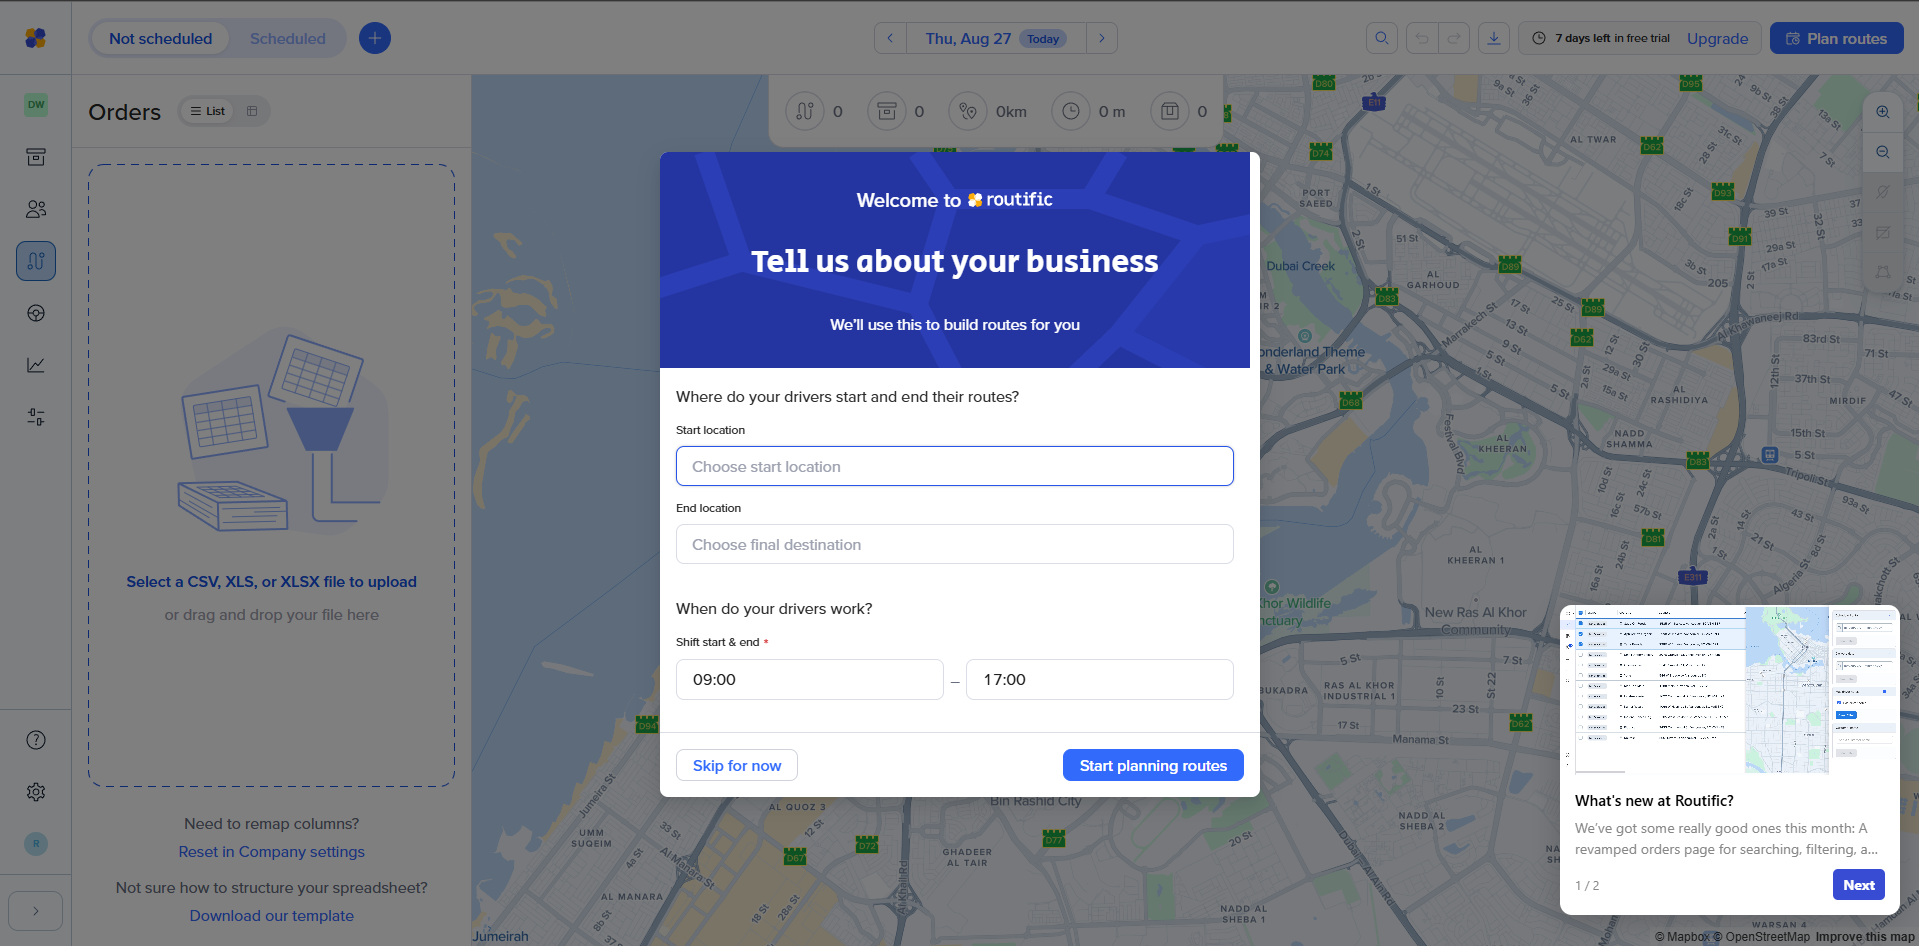
\includegraphics[width=\dimexpr\linewidth-2\fboxsep-2\fboxrule\relax,keepaspectratio]{Images/Routific/Home_Page.png}}}
        \caption{Routific main dashboard view.}
        \label{fig:routific_main}
    \end{subfigure}
    \hfill
    \begin{subfigure}[t]{0.32\textwidth}
        \centering
        \hspace*{0.35cm}{%
            \setlength{\fboxsep}{1pt}%
            \setlength{\fboxrule}{0.5pt}%
            \fbox{
\includegraphics[height=7cm,keepaspectratio]{Images/Routific/Sidebar.png}}%
        }
        \caption{Routific navigation sidebar.}
        \label{fig:routific_sidebar}
    \end{subfigure}
    \caption{Routific capacity and time window interface.}
    \label{fig:routific_capacity}
\end{figure}
%Basically what this does is it combines Home_Page.png and Sidebar.png together horizontally like MS365 Word would do.
Figure~\ref{fig:routific_capacity}\subref{fig:routific_main} shows the full-screen dashboard displayed after the user logs in to Routific. The navigation sidebar appears on the left, with the Orders button highlighted to indicate that the order-management workspace is active. A map of Dubai (using OpenStreetMap) is displayed in the background, while input fields in the foreground allow the user to enter each driver's starting location and shift start time.

Figure~\ref{fig:routific_capacity}\subref{fig:routific_sidebar} shows the navigation sidebar displayed when the Routific route-planning interface is opened. It contains the following options, listed from top to bottom:
\begin{enumerate*}[label=(\alph*)]
  \item workspaces,
  \item orders
  \item customers
  \item routes
  \item drivers
  \item insights
  \item route prefrencing
  \item help
  \item company settings
  \item user settings and log out
\end{enumerate*}

\begin{figure}[H]
    \centering
    \begin{subfigure}[t]{0.48\textwidth}
        \centering
        {\setlength{\fboxsep}{1pt}%
         \setlength{\fboxrule}{0.5pt}%
         \fbox{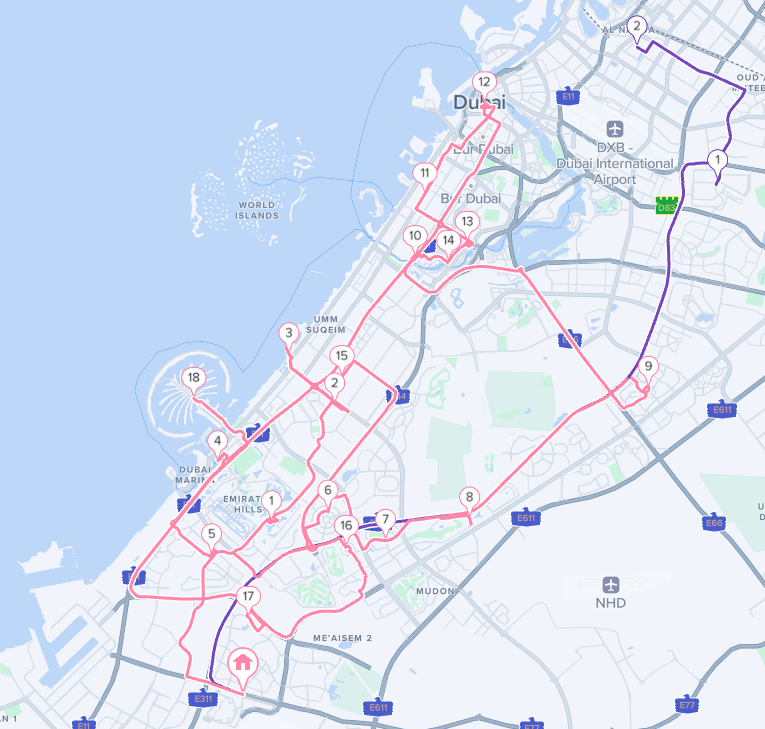
\includegraphics[height=7.05cm,keepaspectratio]{Images/Routific/Optimised Routes Map.png}}}
        \caption{Overall optimised routes map.}
        \label{fig:routific_optimised_map}
    \end{subfigure}
    \hfill
    \begin{subfigure}[t]{0.23\textwidth}
        \centering
        {\setlength{\fboxsep}{1pt}%
         \setlength{\fboxrule}{0.5pt}%
         \fbox{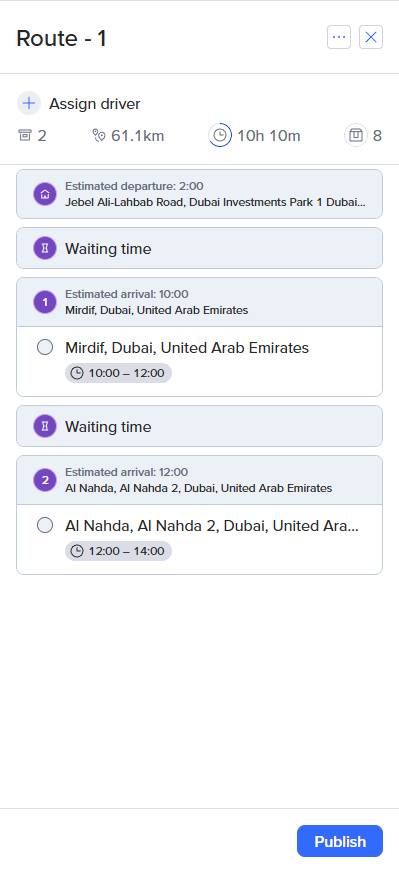
\includegraphics[height=7.05cm,keepaspectratio]{Images/Routific/Optimised_Route_1.png}}}
        \caption{Optimised Route 1.}
        \label{fig:routific_route_one}
    \end{subfigure}
    \hfill
    \begin{subfigure}[t]{0.23\textwidth}
        \centering
        {\setlength{\fboxsep}{1pt}%
         \setlength{\fboxrule}{0.5pt}%
         \fbox{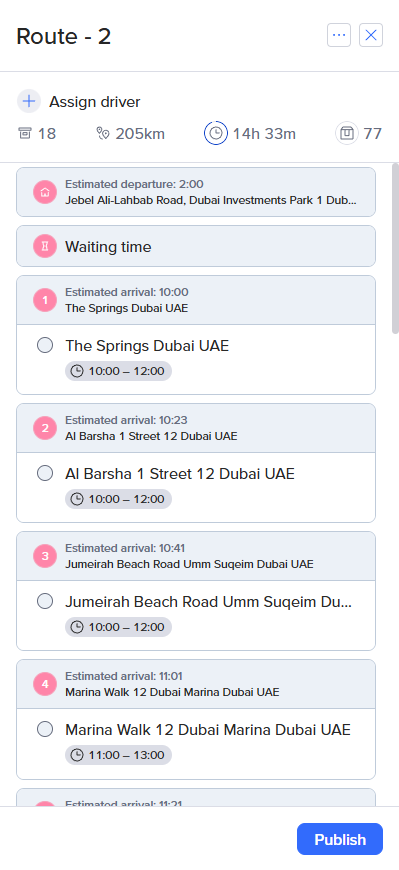
\includegraphics[height=7.05cm,keepaspectratio]{Images/Routific/Optimised_Route_2.png}}}
        \caption{Optimised Route 2.}
        \label{fig:routific_route_two}
    \end{subfigure}
    \caption{Routific's overall optimised route map and the two individual driver routes.}
    \label{fig:routific_optimised_routes}
\end{figure}
To evaluate how commercial solvers handle the constraints identified in Section \ref{Specification} for CVRPTW a test dataset of 20 localized delivery orders was generated and imported into Routific (by using Comma-Seperated Values format). Each record and value was configured with a specific geographic location, a volumetric load value (metric based from 0-10, calculated by mathematical  \(\sum \text{Load\ of\ Assigned\ Orders}\le \text{Vehicle\ Capacity\ Limit}\)) and a strict delivery time window to stress-test the system's scheduling algorithm. A small snippet of the sample data set is provided here.

%VERY IMPORTANT NOTE RAF, U HAVE TO TAKE A NEW SS OF THE OPTIMISED ROUTE 1 AND 2 WITH THE NEW TIMES DO NOT FORGET CUZ LATER IN FINDINGS U USE A NEW SS WITH DIFF TIMES.!!!!!!!!!!!!!!!!!!!!

\begin{table}[H]
\centering
\small
\begin{tabular}{@{}lllc@{}}
\toprule
\textbf{Order ID} & \textbf{Address / Coordinates} & \textbf{Time Window} & \textbf{Load} \\ \midrule
ORD-001 & Dubai Marina, Tower A & 08:00 - 10:00 & 4 \\
ORD-002 & Jumeirah Lakes Towers, Cluster C & 08:30 - 11:00 & 2 \\
ORD-003 & Business Bay, Executive Towers & 10:00 - 12:30 & 5 \\
ORD-004 & Downtown Dubai, Boulevard & 14:00 - 16:00 & 3 \\ \bottomrule
\end{tabular}
\caption{Sample extract of the custom CSV dataset imported into Routific (see Appendix~\ref{app:routific_sample_data} for the full dataset).}
\label{tab:csv_sample}
\end{table}

%Figure~\ref{fig:routific_route_two}\subref{fig:routific_optimised_map} = Figure 2ca??
Figure~\ref{fig:routific_optimised_map} together showcases the algorithm's result of the automatic "Schedule all" optimisation. Both Figure~\ref{fig:routific_optimised_routes}\subref{fig:routific_route_one} and Figure~\ref{fig:routific_optimised_routes}\subref{fig:routific_route_two} contain the following headlined metrics: 
\begin{table}[H]
\centering
\small
\begin{tabular}{@{}lccc@{}}
\toprule
\textbf{Metric} & \textbf{Overall} & \textbf{Optimised Route 1} & \textbf{Optimised Route 2} \\ \midrule
Routes       & 2                   & 1                            & 1                            \\
Orders       & 20                  & 2                            & 18                           \\
Distance     & 266.07 km           & 61.1 km                      & 205 km                       \\
Working time & 24 h 43 min / 31 h  & 10 h 10 min / 15 h 30 min    & 14 h 10 min / 15 h 30 min    \\
Capacity & 85                & 8                            & 77                           \\ \bottomrule
\end{tabular}
\caption{Summary of Routific's overall optimisation and individual route metrics.}
\label{tab:routific_route_metrics}
\end{table}

\subsubsection{Findings}
The solution generated by Routific's inbuilt algorithm unveiled a substancial imbalance between the two drivers. Optimised route 1 (Figure~\ref{fig:routific_optimised_routes}\subref{fig:routific_route_one}) was assigned only 2 of the 20 orders, a combined load of 8 and a distance of 61.1 kilometres. In stark contrast, Optimised route 2 recieved the remaining 18 orders, a combined load of 77 and approximately 205 kilometres. Although every order was allocated and two routes were made, the workload was not distributed evenly as Optimised route two contained 90\% of the orders and around 91\% of the total load. This imbalance is notable given the driver welfare concerns raised in Section \ref{sec:background}. An optimised route allocation system that minimises total distance without workload balance risks reproducing the same over-burdening dynamics aformentioned by concentrating the pressure onto the drivers. 

Furthermore, Routific also produced a solution using only two drivers, although the dataset only contained order information and did not itself establish a set amount of drivers or that 2 drivers would be an appropriate fleet size. This sudgests that the number of avaliable drivers in Optimised route map (Figure~\ref{fig:routific_optimised_routes}\subref{fig:routific_optimised_map}) may have been infered by the route-planning algorithm rather than calculeted from the imported orders. Consequently, a system designed for the intended client should require the fleet size, vehicle capacities and driver shift limits to be entered explicitly rather than anticipation or estimation. To determine whether this result was a of a single occurrence, I submitted the same dataset again again. Routific reproduced the exact same two layouts and the same uneven distributions. I also altred the drivers' shift times but the imbalance remained. Reproducing the results under an altered conditions provides evidance that the outcome was not an isolated anomaly but may instead be caused by Routific's internal processes. 

The difference in working time was also of concern. One driver was given a comparatively small number of deliveries (2) and a long period without any deliveries being made, yet was allocated approximately 9 hours of working time. As an independent comparison, I entered the locations assigned to Optimised Route 2 into Google Maps. At the time of capture and under low-traffic conditions, Google Maps estimated a total driving time of approximately 53 minutes, as shown in Figure~\ref{fig:routific_time_comparison}\subref{fig:google_maps_drive_time}. This estimate is not directly equivalent to Routific's working-time figure because the systems use different path-finding methods and Google Maps does not include service durations, waiting for time windows or breaks. Nevertheless, the large difference suggests that a significant proportion of the scheduled time resulted from waiting and scheduling constraints rather than transportation alone. The break periods allocated by Routific are shown in Figure~\ref{fig:routific_time_comparison}\subref{fig:routific_break_times}.

Another potential source of error is geographic ambiguity. Different streets, buildings or districts may share the same or a very similar name, meaning that an incomplete address could be matched to the wrong coordinates. As demonstrated in Figure~\ref{fig:routific_time_comparison}\subref{fig:routific_geographic_mixup}, this could place a delivery in an unintended location and consequently distort the calculated distance, journey time and allocation of orders between drivers. To reduce this risk, my system should geocode and validate every address before route planning begins. Where multiple matches are found, it should display the standardised address and map location for user confirmation, request additional information such as an area name or coordinates, and prevent optimisation until the ambiguity has been resolved.



\begin{figure}[H]
    \centering
    \begin{subfigure}[t]{0.94\textwidth}
        \centering
        {\setlength{\fboxsep}{2pt}%
         \setlength{\fboxrule}{0.5pt}%
         \fbox{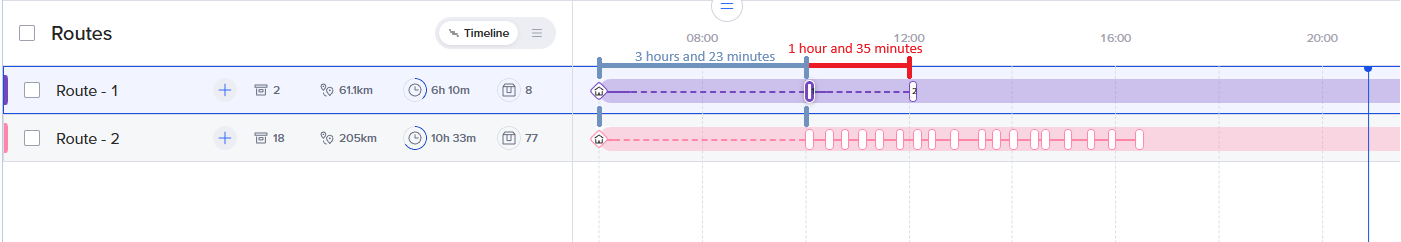
\includegraphics[width=0.97\linewidth]{Images/Routific/Optimised Routes 1 and 2 with break times showing.png}}}
        \caption{Routific schedules for both routes, including the allocated break periods.}
        \label{fig:routific_break_times}
    \end{subfigure}

    \vspace{0.8em}

    \begin{subfigure}[t]{0.46\textwidth}
        \centering
        {\setlength{\fboxsep}{2pt}%
         \setlength{\fboxrule}{0.5pt}%
         \fbox{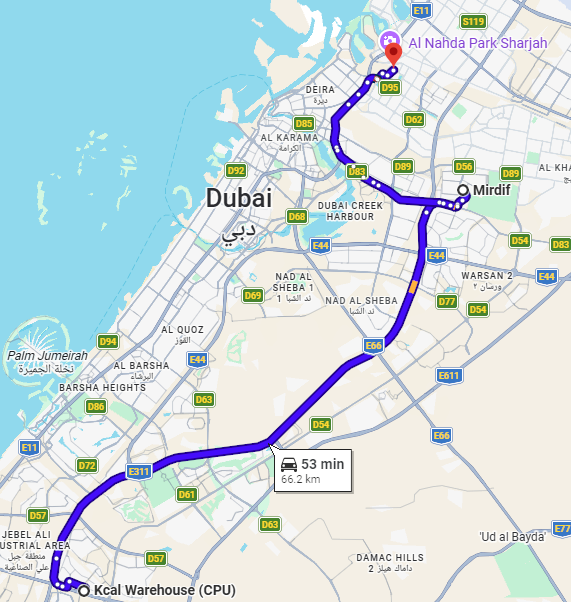
\includegraphics[height=6.6cm,keepaspectratio]{Images/Routific/Google Maps Average Drive Time.png}}}
        \caption{Independent Google Maps estimate of approximately 53 minutes under low-traffic conditions.}
        \label{fig:google_maps_drive_time}
    \end{subfigure}
    \hfill
    \begin{subfigure}[t]{0.46\textwidth}
        \centering
        {\setlength{\fboxsep}{2pt}%
         \setlength{\fboxrule}{0.5pt}%
         \fbox{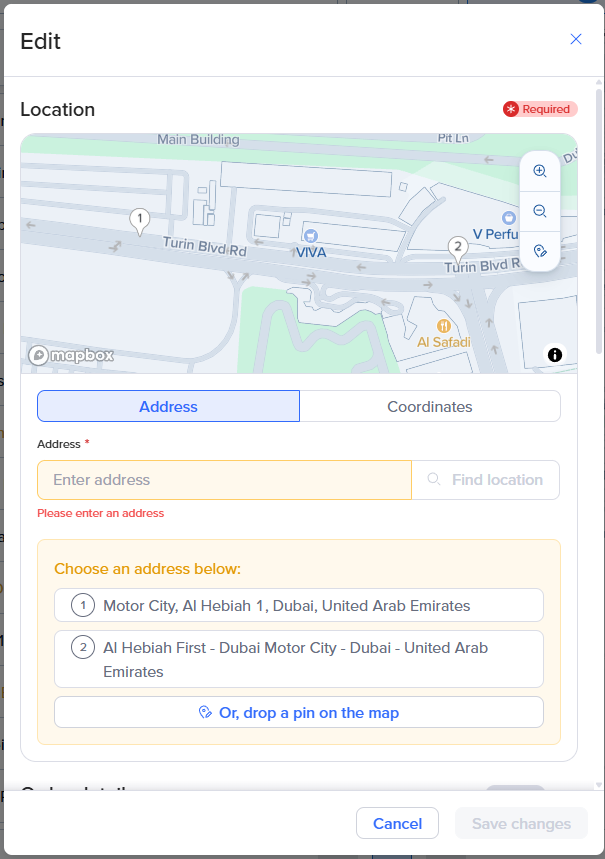
\includegraphics[height=7.8cm,keepaspectratio]{Images/Routific/Geographic mixup.PNG}}}
        \caption{Geographic mix-up identified in Routific's generated route allocation.}
        \label{fig:routific_geographic_mixup}
    \end{subfigure}
    \caption{Comparison of Routific's generated schedules with independent driving-time and geographic evidence.}
    \label{fig:routific_time_comparison}
\end{figure}

\subsubsection{Summary of Routific Analysis}
\label{sec:summary}
The investigation identified several design choices that may make Routific unsuitable for the intended small-business client and that should be addressed differently in my own system:

\begin{enumerate}
    \item \textbf{Workload imbalance.} Routific produced routes containing 2 and 18 stops respectively, with no visible mechanism for balancing work between drivers. My optimisation method should therefore penalise large differences in stop count and allocated load, rather than considering only the total distance or overall fleet load.
    \item \textbf{Capacity applied after route construction.} In the observed workflow, routes were clustered before a specific driver and vehicle capacity were attached. This creates uncertainty over whether an existing route will be rejected or rebuilt when the assigned vehicle has insufficient capacity. My system should check vehicle capacity while constructing and improving each route, rather than treating it as a downstream assignment problem.
    \item \textbf{Manual geographic resolution.} Ambiguous addresses required the user to identify and correct the selected map location manually. My system should detect multiple geocoding matches before optimisation and require the user to confirm the intended address or coordinates.
    \item \textbf{Subscription access.} The interface displayed a limited free trial and an ``Upgrade'' prompt, indicating that continued use requires a paid subscription. This may be a barrier for a small meal-prep business, whereas the proposed bespoke system would not impose a recurring software-subscription charge on the client.
\end{enumerate}

These findings show that an effective route is not defined by distance alone. For the intended client, route validity, balanced driver workloads, reliable address validation and affordable access must also be treated as important system requirements for end-user satisfaction.



\subsection{Evaluation of Pre-existing Systems}
Having conducted an in-depth empirical evaluation of Routific in Section~\ref{sec:routific_analysis}, this section situates those findings alongside the other systems considered in this project's existing-systems research. It is important to distinguish between the depth of evidence available for each system: the findings on Routific are based on direct hands-on testing, including a custom dataset, repeated trials and cross-verification against independent data. Route4Me and Google OR-Tools were not tested directly, so their entries below reflect capabilities stated in their providers' official documentation.\cite{google_ortools_capacity_constraints,google_ortools_time_windows,route4me_capacity_optimisation,route4me_time_windows}
\begin{table}[H]
\centering
\small
\begin{tabular}{@{}p{2.5cm}p{2.5cm}p{2.2cm}p{2cm}p{2.2cm}p{3.2cm}@{}}
\toprule
\textbf{System} & \textbf{Approach} & \textbf{Handles capacity/time windows?} & \textbf{Cost/access} & \textbf{Relevant strength} & \textbf{Relevant limitation (for your user)} \\ \midrule
OR-Tools & Constraint programming and metaheuristics & Yes: capacity constraints and time windows are configurable\cite{google_ortools_capacity_constraints,google_ortools_time_windows} & Free, but requires developer integration & Industry-strength solver & Not directly usable by a non-technical coordinator; it is a library rather than a complete product \\ \midrule
Routific & SaaS & Capacity was applied after clustering in the observed workflow (Section\ref{sec:summary}); time windows produced unexplained idle time (Figure~\ref{fig:routific_time_comparison}\subref{fig:routific_break_times}) & Subscription & Polished interface and dispatch features & Ongoing cost and the workload imbalance identified during direct testing \\ \midrule
Route4Me & SaaS & Provider documentation states that capacity and time-window constraints are supported\cite{route4me_capacity_optimisation,route4me_time_windows} & Commercial access & Supports configurable operational constraints & Not tested directly; some constraint features must be enabled separately \\ \midrule
Manual planning (spreadsheet or WhatsApp) & N/A & No automated checking or built-in route optimiser.  & Free & Familiar and requires no setup & Error-prone, does not scale and matches the interview's reported pain points \\ \bottomrule
\end{tabular}
\end{table}

% Retained for possible later use; excluded from the compiled document.
\begin{comment}
\begin{lstlisting}[style=vscode,caption={Google OR-Tools example demonstrating time-window and waiting-time constraints.},label={lst:ortools_time_windows}]
#Example of Google-OR tools handling capacity and time windows 
# 1. Register the time callback (travel time + service time)
time_callback_index = routing.RegisterTransitCallback(time_callback)

# 2. Add the time dimension (enabling slack/waiting time)
routing.AddDimension(
    time_callback_index,
    60,  # max allowed waiting time (slack)
    1440, # max total travel time per vehicle (capacity)
    False, # Don't force start time cumulative to zero
    "Time"
)
time_dimension = routing.GetDimensionOrDie("Time")

# 3. Apply individual time windows to specific location indexes
for location_idx, time_window in enumerate(data['time_windows']):
    index = manager.NodeToIndex(location_idx)
    time_dimension.CumulVar(index).SetRange(time_window[0], time_window[1])

\end{lstlisting}
\end{comment} 
%held in a comment so it is usefull to copy later but will not effect the code now

\subsection{Client Interview}
Understanding my client's environment directly informs the design of a more reliable and usable product. I interviewed the dispatch manager of a local daily meal-prep delivery business to establish operational constraints and functional requirements.

\newcommand{\rangeofdeliveries}{40 to 60}
\newcommand{\numberofvehicles}{three delivery vans.}

\begin{enumerate}[label={\LARGE Q\arabic*\,}]
    \item \textbf{What would you like the program to do?} \\
    \textit{Client:} "Basically, I need a tool where I can upload our daily customer meal drop-offs—usually~\rangeofdeliveries- addresses and automatically split them between our~\numberofvehicles~. Right now, doing it by hand takes forever because we have tight morning delivery slots, and I need to make sure no van gets overloaded or sent back and forth across Dubai."

%we are using vans for this scenario. maybe i will swtich to motorcycles and a lower amount of set 

    \item \textbf{What tools have you used for route planning in the past, and where do they fall short?} \\
    \textit{Client:} "We mostly rely on a massive Google Sheet and WhatsApp groups to send stops to drivers. We tried commercial software like Routific, but subscription costs add up fast for a small team, and it often creates unbalanced routes—like giving one driver 18 stops and another only 2—without considering driver workload fairness."

    \item \textbf{What specific features would make route optimization easier for your daily operation?} \\
    \textit{Client:} "It has to respect vehicle load capacity—our vans carry a maximum of 20 to 25 bag meals. Also, time windows are critical: premium clients expect their breakfast bags between 6:00 AM and 8:00 AM. The program must flag any delivery that cannot be made on time rather than silently failing."

    \item \textbf{What do you particularly enjoy about your current method that we should keep?} \\
    \textit{Client:} "Our drivers know Google Maps inside out. They don't want to learn a complex new navigation app. If your system can generate the optimal sequence and let me push the final route directly to their phones via a Google Maps link or export, that would fit perfectly into how we already work."

    \item \textbf{Would features like manual route adjustment and load-balancing sound useful to incorporate?} \\
    \textit{Client:} "Absolutely. Sometimes a driver calls in sick or road closures happen near downtown. Being able to manually swap a stop between drivers or tweak the sequence on a visual interface before locking it in would be a lifesaver."

    \item \textbf{How do you currently verify that a route plan is practical before drivers hit the road?} \\
    \textit{Client:} "Honestly, it's just guesswork and experience. A good system should clearly show total distance, estimated route duration, and highlight any capacity or time-window violations before we dispatch."
\end{enumerate}

\subsubsection{Interview Summary}
Based on the interview, my client has expressed a need for an automated routing optimisation solution that directly tackles the inefficencies of manual route planning. The solution must ensure balanced routes and workload fairness while actively respecting capacity constraints. The client articulated that the system must accomidate for premium customer time limitations while blatantly signaling any time collisions in the system. The application should generate optimised routes and transmit the data onto a familiar navigation application (the client explicitly mentioned Google Maps) and communicated the adequacy of the existing system. Another articulation that was expressed was the need for manual route adjustments and the ability to swap stops between drivers and manipulate the sequence orders on a user-friendly graphical user interface. The final comment is that the system must display practical data (such as total distance, estimated route duration and the highlighting of capacity or time violations) in a manner that is unambiguous. 



\subsection{Legal, Ethical and Data Protection Considerations}
The processes illustrated in Figure~\ref{fig:ipos_chart} and Appendix~\ref{app:visual_flowchart} may involve collecting, processing and storing information that identifies individual customers or drivers. Privacy, responsible data handling and the protection of this information must therefore be considered throughout the design and development of the solution. This section outlines the relevant legal, ethical and data protection considerations.

\subsubsection{Data Protection and Privacy}
The solution may handle the following categories of information:
\begin{enumerate}
    \item Customer names or identification numbers.
    \item Delivery addresses.
    \item Telephone numbers.
    \item Order histories.
    \item Precise locations of drivers and customers.
    \item Driver identities.
    \item Driver performance records.
\end{enumerate} 
Where these records identify an individual, either directly or when combined with other information, they may constitute personally identifiable information (PII) under NIST guidance or personal data under the GDPR.\cite{nist_sp_800_122,eu_gdpr_2016}. The system should therefore collect only the information needed for its intended functions and protect it against unauthorised access, disclosure or misuse.

I will design the system to only collect and retain personal information that is strictly necessary for route optimisation. I will also implement the following: 

\begin{enumerate}
    \item Encryption at rest and in transit
    \item Irreversable hashing algorithms 
    \item Authentication and role-based access rights
    \item Limited data retention
    \item Anonymised customer and driver identifiers
    \item Audit logs
    \item Clear explication of what data is collected and why.
\end{enumerate} 

\subsubsection{Algorithmic Fairness}
As the soultion may integrate a tiered service and deliberately prioritise one class of customers over others (second-degree price discrimination). Courts and regulatory bodies globally recognize this as inherently legal, because the difference in treatment is justified by a corresponding difference in financial consideration, however this system may treat similar customers differently (which voilates the basic notion of distributive justice and fairness). I will avoid this by concreating the premium service to offer an earlier delivery window while not overriding the driver safety or the promise made to other customers. I will ensure to protect every customer's agreed delivery window, while allowing narrower windows purchased by premium customers and I will 

Futhermore, another cuase of concern may be the solutions ability to record drivers average speeds compared to a baseline, for example 
\[
\left.
\begin{aligned}
&\text{Driver A = 1.2x} \\
&\text{Driver B = 1.0x} \\
&\text{Driver C = 0.8x}
\end{aligned}
\right\} \text{where the baseline speed ($x$) is being multiplied by the coefficents}
\]
If the solution were to then give the driver with the fastest speeds (driver A in this case), this may overload the drivers (which this solution is ment to reduce). Therefore, I must distinguish between optimisation efficiency and maximising workload for the fastest employee (as shown in \ref{fig:routific_capacity}\subref{fig:routific_main}). To solve this, the solution may introduce a constraint such as $\text{Workload}_{\max} - \text{Workload}_{\min} < L$ or constrict the number of deliveries or hours to a set maximum. 

The measure of relative speed is also a cuase for ethical concern as it may not be a fair measure of efficeincy. This is becuase a driver may appear slow due to factors which he may not be able to control.
 
\begingroup
\renewcommand{\arraystretch}{1.25}
\noindent
\begin{tabular}{@{}L{0.46\linewidth}@{\hspace{0.08\linewidth}}L{0.46\linewidth}@{}}
\textbullet\ Vehicle differences & \textbullet\ Traffic \\
\textbullet\ Road restrictions & \textbullet\ Weather \\
\textbullet\ Delivery area characteristics and temporary circumstances & \\
\end{tabular}
\par
\endgroup

\subsubsection{Supervision and Oversight}
The system should support, rather than replace, the judgement of a delivery coordinator. Its recommendations will depend on the data and constraints provided, which may not capture unexpected disruptions or operational knowledge available to the dispatcher. An authorised dispatcher should therefore be able to review the generated plan before dispatch and:

\begin{itemize}
    \item Override a suggested route or adjust the order of its stops.
    \item Reassign an order to another driver.
    \item Remove an unavailable driver from the active fleet and reallocate affected deliveries.
    \item Change delivery priorities while respecting agreed delivery windows.
    \item Lock selected delivery assignments so that subsequent optimisation preserves them.
    \item Reject the generated solution and request a revised plan.
\end{itemize}

Manual control should not bypass the checks used to establish route validity. After any adjustment, the system should recalculate route metrics and check vehicle capacity, delivery windows and driver shift limits. Any violations or unallocated deliveries should be clearly highlighted, and an invalid plan should not be approved for dispatch. Changes should also be recorded in an audit log so that decisions can be reviewed and responsibility remains clear.

\subsubsection{Driver Health, Safety and Employment}
As discussed in Section~\ref{sec:background}, the driver welfare concerns motivating this project include long working hours, exposure to extreme heat, fatigue and financial pressure to complete more deliveries. That discussion also highlights how performance-based pay and algorithmic pressure may encourage unsafe driving when delays threaten earnings. The workload imbalance identified during the Routific investigation, summarised in Section~\ref{sec:summary}, showcase long continous drive times with little to no breaks. While this may be efficient computationally, it may constitute to an unhealthy lifestyle. To mitigate this, I will introduce mandatory breaks into the solution.   

\newpage
\section{Design}

\subsection{Data Specification}
\subsubsection{Data Dictionary}

\begin{table}[H]
\centering
\small
\renewcommand{\arraystretch}{1.2}
\begin{tabular}{@{}L{2.5cm}L{1.6cm}L{4.2cm}L{3.8cm}L{2.2cm}@{}}
\toprule
\textbf{Variable} & \textbf{Data Type} & \textbf{Validation / Constraints} & \textbf{Purpose / Description} & \textbf{Example} \\ \midrule
\code{studentName} & String & Must not be empty; alphabetic characters only & Stores the student's name & ``Ahmed Ali'' \\ \bottomrule
\end{tabular}
\end{table}

\subsubsection{Data Volumes Estimations}

\begin{table}[H]
\centering
\small
\renewcommand{\arraystretch}{1.2}
\begin{tabular}{@{}L{2.5cm}L{3.0cm}L{3.8cm}L{2.6cm}L{2.4cm}@{}}
\toprule
\textbf{Data Item} & \textbf{Description} & \textbf{Estimated Size per Use (\unit{\kilo\byte})} & \textbf{Frequency Estimate} & \textbf{Total Volume (Daily)} \\ \midrule
studentName & String & Must not be empty; alphabetic characters only & Stores the student's name & ``Ahmed Ali'' \\ \bottomrule
\end{tabular}
\end{table}

\subsection{Evaluation of Algorithms}
Capacitated Vehicle Routing Problem (CVRP) is solved using three main families of algorithms: exact algorithms, classical heuristics, and metaheuristics/hybrid methods. Evaluating and comparing these changes 

\subsubsection{Exact Algorithms}
Exact algorithms guarantee the absolutle mathematically optimal route, however they are notoriously slow as the number of parameters (delivery locations) grow. 

\begin{enumerate}
    \item \textbf{Branch-Cut-and-Price (BCP).} Combines branch-and-bound, cutting planes, and column generation. It is a well-established exact approach for CVRP: \textcite{pecin2017improved_bcp} solved all instances in their benchmark set with up to 199 customers, as well as some larger instances with up to 360 customers. These are experimental results, not a guaranteed problem-size limit.

    \textbf{Time complexity:} implementation-dependent, with a binary search tree of depth $d$ containing up to $\mathcal{O}(2^d)$ nodes and nonconstant work per node; see Appendix~\ref{app:complexity_bcp} for the calculation and assumptions.
    \item \textbf{Mixed-Integer Programming (MIP).} Formulates the routing problem with mathematical equations and integer variables. It works well for very small sets (under 50 locations) but struggles to scale.
\end{enumerate}

\subsubsection{Classical Heuristics}
Heuristics are fast, rule-based procedures that quickly build a practical route without guaranteeing optimality. They often follow a cluster-first, route-second or route-first, cluster-second design.

\begin{enumerate}
    \item \textbf{Nearest-Neighbour (NN) Construction.} Starting from the depot, the vehicle repeatedly travels to the closest unvisited customer that does not violate the current constraints (capacity, time window), until no further customer can be added, at which point the vehicle returns to the depot and, if unserved customers remain, a new route is started. NN is simple to implement, easy to reason about and debug, and naturally extends to include constraint checks at the point of construction rather than as an afterthought -- directly addressing the capacity-applied-after-construction weakness identified in Routific (Section~\ref{sec:summary}). Its principal disadvantage is short-sightedness: a locally optimal choice early in the route can force a long, inefficient "straggler" journey later, typically producing routes 15--25\% longer than optimal.\cite{ref_nn_performance}. 

    \textbf{Time complexity:} $\mathcal{O}(n^2)$ for the basic nearest-neighbour scan over $n$ vertices; see Appendix~\ref{app:complexity_nn} for the derivation and assumptions.

    \item \textbf{Clarke-Wright Savings Algorithm.} Begins by assigning every customer their own individual round-trip route from the depot, then iteratively merges pairs of routes that yield the greatest "saving" in total distance, provided the merge does not violate vehicle capacity. Savings tends to outperform NN on solution quality and is a long-standing industry-standard heuristic, but it is more involved to implement correctly (it requires computing and re-sorting a savings list of every customer pair, and re-checking feasibility after every merge) and its natural formulation targets capacity constraints more directly than time windows, which would need to be retrofitted as an additional feasibility check on each candidate merge.\cite{ref_clarke_wright}

    \textbf{Time complexity:} $\mathcal{O}(n^2\log n)$ for $n$ customers under the implementation assumptions in Appendix~\ref{app:complexity_savings}, with sorting the savings list dominating the cost.

    \item \textbf{Sweep Algorithm.} Customers are first clustered by sweeping a rotating ray from the depot and grouping consecutive customers into a cluster until a vehicle's capacity is reached (cluster-first), after which a route is optimised within each cluster (route-second), often using NN or a TSP solver. Sweep is intuitive for capacity constraints and produces visually sensible route clusters, but does not naturally incorporate time windows into the clustering step, and its solution quality is sensitive to the depot's position relative to the customers.\cite{gillett1974heuristic}

    \textbf{Time complexity:} $\mathcal{O}(n^2)$ for $n$ customers under the implementation assumptions in Appendix~\ref{app:complexity_sweep}, with sorting the savings list dominating the cost.
\end{enumerate}

\subsubsection{Metaheuristics and Hybrid Methods}
Metaheuristics wrap a constructive heuristic with an iterative improvement process to escape local optima and approach near-optimal solutions.

\begin{enumerate}
    \item \textbf{2-opt / Or-opt Local Search.} Given an existing route, 2-opt repeatedly reverses a segment of the route if doing so reduces total distance, removing "crossed" paths; Or-opt similarly relocates short chains of one to three consecutive customers to a better position. Both are simple to layer on top of any constructive heuristic (including NN) as a post-processing improvement step, and are computationally cheap for realistic instance sizes (tens of customers).\cite{ref_2opt}

    \item \textbf{Genetic Algorithms (GA) / Simulated Annealing (SA) / Tabu Search.} These maintain a population (GA) or a single evolving solution (SA, Tabu) and apply randomised or memory-guided moves across many iterations to search a much larger portion of the solution space than local search alone, typically producing solutions closer to optimal than a constructive heuristic with a simple local search. Their cost is implementation and tuning complexity: each requires careful parameter selection (mutation rate, cooling schedule, tabu tenure), longer development time, and is considerably harder to debug when a route is invalid, since the fault could lie in the move operator, the fitness function, or the constraint-checking logic.\cite{ref_metaheuristics}
\end{enumerate}

\subsubsection{Comparison of Candidate Approaches}
\begin{table}[H]
\centering
\small
\begin{tabular}{@{}L{2.6cm}L{2.6cm}L{2.6cm}L{2.6cm}L{3.4cm}@{}}
\toprule
\textbf{Algorithm} & \textbf{Solution quality} & \textbf{Implementation complexity} & \textbf{Ease of extending to capacity/time windows} & \textbf{Suitability given project constraints} \\ \midrule
Exact (BCP/MIP) & Optimal & Very high & High (constraints are declared, not coded) & Unsuitable: impractical to implement from scratch within an A-level timeframe, and does not scale to the client's 40--60 daily orders \\ \midrule
Nearest-Neighbour & Low--moderate & Low & High -- constraints checked directly at each construction step & Strong fit: matches current skill level, fast to implement and test, directly solves the Routific capacity-timing flaw \\ \midrule
Clarke-Wright Savings & Moderate--high & Moderate--high & Moderate -- time windows require retrofitting & Weaker fit: meaningfully better quality, but a higher implementation and debugging cost for the remaining time available \\ \midrule
Sweep & Moderate & Moderate & Low for time windows & Weaker fit: clustering step does not map cleanly onto the client's strict morning windows \\ \midrule
2-opt (as improvement) & Improves any of the above & Low--moderate & N/A (post-processing) & Strong fit: cheap to add on top of NN once NN is working and tested \\ \midrule
GA / SA / Tabu Search & High & Very high & Moderate--high, but adds further tuning complexity & Unsuitable as a primary method: highest risk of an incomplete or unreliable Technical Solution given available development time \\ \bottomrule
\end{tabular}
\caption{Comparison of candidate CVRPTW algorithms against project constraints.}
\label{tab:algorithm_comparison}
\end{table}


\subsubsection{Conclusion and Justification}
An exact algorithm was rejected outright: Branch-Cut-and-Price and MIP formulations guarantee optimality but require solver expertise and computation time that are both incompatible with a single-developer A-level project and a client dataset of 40--60 daily orders.

Of the remaining heuristics, this project will use a \textbf{nearest-neighbour construction heuristic, extended with capacity and time-window feasibility checks applied at each step of construction, followed by a 2-opt local search as a route-improvement stage}. This decision was reached against three explicit criteria rather than a single preference:

\begin{enumerate}
    \item \textbf{Correctness and debuggability over marginal solution quality.} A route that reliably respects every capacity and time-window constraint is of greater practical value to the client than a marginally shorter route that occasionally produces an invalid plan. Section~\ref{sec:summary} identified exactly this trade-off as a weakness in Routific: my system should check feasibility \textit{during} construction rather than as a downstream step. Nearest-neighbour is the most direct heuristic in which to embed that check, since candidate customers can simply be excluded from consideration the moment they would violate a constraint.
    \item \textbf{Development time and risk.} With deadlines from other qualifications competing for the same time as this NEA, a heuristic that can be implemented, tested and debugged correctly is of more value than a more sophisticated metaheuristic that risks being incomplete or unreliable at submission. Clarke-Wright and Sweep were considered as moderate-complexity alternatives with better solution quality, but were judged to carry a higher implementation cost for the remaining project time relative to their benefit, particularly given that time windows are not a natural fit for either method without additional retrofitting.
    \item \textbf{A staged path to a higher mark band.} 2-opt is retained as a planned improvement stage precisely because it can be added \textit{after} a correct, tested nearest-neighbour baseline exists, without requiring that baseline to be rewritten. This allows the project to demonstrate a working, constraint-respecting baseline early, then extend it -- an approach that is both lower-risk and, if time allows, gives the option of implementing and evaluating an additional metaheuristic (e.g. simulated annealing) as a stretch objective for comparison against the baseline in the Evaluation section, rather than as a required deliverable the whole system depends on.
\end{enumerate}



\subsection{Visualisation of system processes}
\subsubsection{System Process Visualisation}

\begin{figure}[H]
    \centering
    
    \setlength{\fboxsep}{5mm}%
    \setlength{\fboxrule}{0.5pt}%
    \makebox[\linewidth][c]{\fbox{\includegraphics[width=1.07625\linewidth,height=0.861\textheight,keepaspectratio]{Images/Flowcharts/Frame 2.pdf}}}
    \caption{System process flowchart.}
    \label{fig:system_process_flowchart}
\end{figure}

The creation of a flowchart for the purposes of visualising the processes of the intended soultion has been a useful approach is it has allowed clear visalisation and decomposition of abstract processes and illustration of sequences of processes. The flowchart will also help during the development of the solution as it acts as a potential blueprint and can help identify inefficiencies and logical errors before execution and development. Note that capacity and time-window admission happen inside Construct routes, and Check constraints validates only whole-plan feasibility (unallocated stops, route-level limits)

\subsubsection{Information Processing Cycle}

\begin{figure}[H]
    \centering
    \makebox[\linewidth][c]{\includegraphics[width=1.1\linewidth,keepaspectratio]{Images/Flowcharts/ipos_chart.pdf}}
    \caption{Input, processing, output and storage (IPOS) cycle.}
    \label{fig:ipos_chart}
\end{figure}

To further reinforce the benifits of visualising the processes of the solution, I have created an IOPS chart to showcase how raw input data transforms by processes to outputs and where it may be saved in, it also allows me to visualise potential missing steps or unaccounted errors in the solution.    

\subsubsection{Visualisation of Flow of Data}

\begin{figure}[H]
    \centering
    \makebox[\linewidth][c]{\includegraphics[width=1.1\linewidth,keepaspectratio]{Images/Flowcharts/Blank_diagram_padded.pdf}}
    \caption{Data flow through the route allocation system.}
    \label{fig:data_flow}
\end{figure}


The diagram summarises how order and vehicle data move through the system. The delivery coordinator provides the initial records, which are validated and geocoded before a distance--time matrix is produced. Routes are then constructed, checked against the system constraints and improved before their metrics and warnings are displayed. The coordinator may manually adjust the proposed routes, after which they are checked again, while the final route results and audit information are stored for future review.

%%%%%%%%%%%%%%%%%%%%%%%%%%%%%%%%%%%%%%%%%%%%%%%%%%%%%%%%%%%%%%%%%%%%%%%%%%%%%%%%%%%%%%%%%%%%%
% start of refrences
\newpage
\printbibliography



\newpage
\begin{appendices}
%This is the beginning of the appendix

\section{Routific Sample Data}
\label{app:routific_sample_data}
This appendix contains the unedited sample data imported into Routific's automated route allocation system. The resulting routes are shown in Figure~\ref{fig:routific_optimised_routes}.
\begin{landscape}
\begin{longtable}{@{}L{1.8cm}L{6cm}L{1.6cm}L{1.6cm}L{1.3cm}L{2.4cm}L{5.6cm}@{}}
\caption{Routific Sample Order Data} \label{tab:routific_sample_data} \\
\toprule
\textbf{Order} & \textbf{Address} & \textbf{Start} & \textbf{End} & \textbf{Load} & \textbf{Duration (mins)} & \textbf{Notes} \\
\midrule
\endfirsthead

\toprule
\textbf{Order} & \textbf{Address} & \textbf{Start} & \textbf{End} & \textbf{Load} & \textbf{Duration (mins)} & \textbf{Notes} \\
\midrule
\endhead

\midrule
\multicolumn{7}{r}{\textit{Continued on next page}} \\
\endfoot

\bottomrule
\endlastfoot

Order 1  & Marina Walk 12, Dubai Marina, Dubai, UAE      & 11:00 & 13:00 & 4 & 5  & Vegetarian meal boxes \\
Order 2  & Al Wasl Road 45, Jumeirah 1, Dubai, UAE        & 12:00 & 14:00 & 6 & 5  & Leave with concierge \\
Order 3  & Sheikh Zayed Road, Business Bay, Dubai, UAE    & 11:30 & 13:30 & 3 & 5  & Office delivery, ring bell \\
Order 4  & Al Barsha 1, Street 12, Dubai, UAE              & 10:00 & 12:00 & 5 & 5  & Gate code 4521 \\
Order 5  & Downtown Boulevard, Dubai, UAE                  & 13:00 & 15:00 & 2 & 5  & Call on arrival \\
Order 6  & Jumeirah Beach Road, Umm Suqeim, Dubai, UAE     & 10:00 & 12:00 & 4 & 5  & No pork items \\
Order 7  & Al Quoz Industrial 3, Dubai, UAE                & 14:00 & 16:00 & 8 & 10 & Bulk order for staff canteen \\
Order 8  & Motor City, Dubai, UAE                          & 11:00 & 13:00 & 3 & 5  & Fragile packaging \\
Order 9  & Dubai Silicon Oasis, Dubai, UAE                 & 12:30 & 14:30 & 4 & 5  & Leave at reception \\
Order 10 & Arabian Ranches, Dubai, UAE                     & 10:30 & 12:30 & 5 & 5  & Gluten free meals \\
Order 11 & Al Furjan, Dubai, UAE                           & 13:00 & 15:00 & 3 & 5  & Call before arrival \\
Order 12 & Dubai Sports City, Dubai, UAE                   & 14:30 & 16:30 & 6 & 5  & Weekly subscription box \\
Order 13 & Jumeirah Village Circle, Dubai, UAE             & 11:00 & 13:00 & 2 & 5  & High protein plan \\
Order 14 & Palm Jumeirah, Dubai, UAE                       & 15:00 & 17:00 & 4 & 10 & Villa delivery, gate access needed \\
Order 15 & Mirdif, Dubai, UAE                              & 10:00 & 12:00 & 3 & 5  & Standard plan \\
Order 16 & Al Nahda, Dubai, UAE                            & 12:00 & 14:00 & 5 & 5  & Family size order \\
Order 17 & Deira Creek, Dubai, UAE                         & 13:30 & 15:30 & 4 & 5  & Office building, 3rd floor \\
Order 18 & Dubai Investment Park, Dubai, UAE               & 14:00 & 16:00 & 7 & 10 & Corporate catering order \\
Order 19 & Discovery Gardens, Dubai, UAE                   & 11:00 & 13:00 & 3 & 5  & Vegan plan \\
Order 20 & The Springs, Dubai, UAE                         & 10:00 & 12:00 & 4 & 5  & Standard plan \\

\end{longtable}
\end{landscape}

\begin{landscape}
\section{System Process Visualisation Flowchart}
\label{app:visual_flowchart}
This appendix presents an enlarged version of the system process flowchart in Figure~\ref{fig:system_process_flowchart}, preserving all content and proportions for clearer reading.

\begin{figure}[H]
    \centering
    \includegraphics[width=\linewidth,keepaspectratio]{Images/Flowcharts/Frame 2.pdf}
    \caption{Enlarged system process flowchart.}
    \label{fig:system_process_flowchart_landscape}
\end{figure}
\end{landscape}

\clearpage
\section{Algorithm Time Complexity Calculations}
\label{app:algorithm_complexity}
This appendix presents the calculations supporting the complexity summaries in the algorithm evaluation. The bounds depend on the implementation assumptions stated below.

\subsection{Branch-Cut-and-Price}
\label{app:complexity_bcp}
BCP combines branching with column generation and cutting planes. Processing a search-tree node can require repeated linear-programming solves, pricing searches and cut separation, so its cost is not a single constant-time operation.\parencite{pessoa2020generic_vrp}

For a binary branching implementation, let $d$ be the maximum search-tree depth, with the root at depth zero, and let $B$ be the number of processed nodes. A full binary tree gives the following upper bound:
\[
\begin{aligned}
    B &\le \sum_{j=0}^{d} 2^j \\
      &= 1+2+4+\dots+2^d \\
      &= 2^{d+1}-1.
\end{aligned}
\]
Let $T_{\text{setup}}$ denote preprocessing time and $C_{\text{node}}$ an upper bound on the total work at any processed node, including all pricing and cutting iterations and branching evaluations. Then:
\[
\begin{aligned}
    T_{\text{BCP}} &\le T_{\text{setup}}+B C_{\text{node}} \\
    &\le T_{\text{setup}}+(2^{d+1}-1)C_{\text{node}} \\[0.5em]
    T_{\text{BCP}} &= \mathcal{O}\!\left(T_{\text{setup}}+2^d C_{\text{node}}\right).
\end{aligned}
\]
This is a conditional search-tree bound, not a universal $\mathcal{O}(2^n)$ running time: the depth $d$ is not necessarily the number of customers $n$, and $C_{\text{node}}$ also depends on the instance and implementation. In particular, the generic elementary shortest-path problem with resource constraints, used in vehicle-routing pricing, is strongly NP-hard.\parencite{irnich2006shortest_path} Pruning may substantially reduce the number of nodes actually explored.

Algorithm sources: \textcite{pecin2017improved_bcp,pessoa2020generic_vrp}. The calculation above is a derivation under a binary-branching model, rather than a complexity theorem quoted from these papers.

\subsection{Nearest-Neighbour Construction}
\label{app:complexity_nn}
Given a graph $G = (V, E)$ with $\lvert V\rvert = n$ vertices, the basic nearest-neighbour scan examines each remaining unvisited vertex before selecting the next one. Assuming constant-time distance lookups and candidate checks, the number of candidate examinations is:
\[
\begin{aligned}
    \text{Total Operations} &= \sum_{k=1}^{n-1} (n - k) \\
    &= (n - 1) + (n - 2) + \dots + 1 \\
    &= \frac{n(n - 1)}{2} \\[0.5em]
    \text{Time Complexity} &= \mathcal{O}(n^2).
\end{aligned}
\]
This calculation describes the basic scan; additional route restarts or more expensive feasibility checks must be accounted for separately in the constrained implementation.

Algorithm source: \textcite{Rosenkrantz1977}.

\subsection{Clarke-Wright Savings Algorithm}
\label{app:complexity_savings}
Let $n$ be the number of customers, excluding the depot, and $m$ the number of distinct customer pairs. Each customer is paired with every customer that follows it, so no pair is counted twice:
\[
\begin{aligned}
    m &= \sum_{k=1}^{n-1} (n-k) \\
      &= (n-1)+(n-2)+\dots+1 \\
      &= \frac{n(n-1)}{2} \\[0.5em]
    T_{\text{compute}}(n) &= \mathcal{O}(m)=\mathcal{O}(n^2).
\end{aligned}
\]
Assuming each saving takes constant time to calculate, computing the list is quadratic. Sorting the $m$ savings once with an $\mathcal{O}(m\log m)$ comparison sort then gives:
\[
\begin{aligned}
    T_{\text{sort}}(n) &= \mathcal{O}(m\log m) \\
    &= \mathcal{O}\!\left(\frac{n(n-1)}{2}\log\!\left(\frac{n(n-1)}{2}\right)\right) \\
    &= \mathcal{O}(n^2\log(n^2)) \\
    &= \mathcal{O}(2n^2\log n) \\
    &= \mathcal{O}(n^2\log n).
\end{aligned}
\]
For a single pass through the sorted list, assume that route membership is maintained using disjoint-set union with path compression and union by rank, and that endpoint and capacity checks take constant time. Here, $\alpha(n)$ denotes the inverse Ackermann function associated with the amortised cost of disjoint-set operations. Under these implementation assumptions:
\[
\begin{aligned}
    T_{\text{merge}}(n) &= \mathcal{O}(m\alpha(n)) \\
    &= \mathcal{O}(n^2\alpha(n)) \\[0.5em]
    T_{\text{total}}(n) &= T_{\text{compute}}(n)+T_{\text{sort}}(n)+T_{\text{merge}}(n) \\
    &= \mathcal{O}(n^2+n^2\log n+n^2\alpha(n)) \\
    &= \mathcal{O}(n^2\log n).
\end{aligned}
\]
The sorting term dominates this bound: $n$ is the input size, while $n^2$ describes the growth in the number of pairs, not a maximum value of $n$. Additional checks that scan entire routes, such as recomputing time-window feasibility, would need to be analysed separately.

Algorithm source: \textcite{clarke1964scheduling}. The calculation above is an implementation-dependent complexity analysis.

\subsection{Sweep Algorithm}
\label{app:complexity_sweep}
Let $n$ be the number of customers, excluding the depot. The clustering phase calculates each customer\textquotesingle s polar angle relative to the depot, sorts the customers by angle, then assigns them to routes in a single sweep. Assuming constant-time angle calculations and capacity checks:
\[
\begin{aligned}
    T_{\text{angles}}(n) &= \mathcal{O}(n) \\
    T_{\text{sort}}(n) &= \mathcal{O}(n\log n) \\
    T_{\text{sweep}}(n) &= \mathcal{O}(n) \\[0.5em]
    T_{\text{clustering}}(n) &= T_{\text{angles}}(n)+T_{\text{sort}}(n)+T_{\text{sweep}}(n) \\
    &= \mathcal{O}(n+n\log n+n) \\
    &= \mathcal{O}(n\log n).
\end{aligned}
\]
Optional optimisation within each route has a separate cost. If the $k$ routes contain $m_1,\dots,m_k$ customers, with $\sum_{i=1}^{k}m_i=n$, and the chosen route-ordering heuristic takes $\mathcal{O}(m_i^2)$ time per route, then:
\[
\begin{aligned}
    T_{\text{ordering}}(n) &= \mathcal{O}\!\left(\sum_{i=1}^{k}m_i^2\right), \\
    \sum_{i=1}^{k}m_i^2 &\le \left(\sum_{i=1}^{k}m_i\right)^2=n^2, \\[0.5em]
    T_{\text{total}}(n) &= T_{\text{clustering}}(n)+T_{\text{ordering}}(n) \\
    &= \mathcal{O}(n\log n+n^2) \\
    &= \mathcal{O}(n^2).
\end{aligned}
\]
The $\mathcal{O}(n\log n)$ bound applies to clustering alone. The bound including route ordering depends on the chosen heuristic; it is not a general bound for solving the travelling salesperson problem exactly.

Algorithm source: \textcite{gillett1974heuristic}. The calculation above is an implementation-dependent complexity analysis.



\end{appendices}

\end{document}
